In this chapter we describe how we predict the position of periods, commas and question marks in unpunctuated text using lexical features.
The used data is described in Section \ref{sec:training_data}. 

\subsection{Data Preprocessing}
The system is based on the deep learning framework \emph{caffe}.
Therefore the processing pipeline is the following:

\begin{itemize}
\item pre process the data, so that it can be used as input for caffe
\item learn the network with the preprocessed data
\item predict the new data
\item post process the output, to show a valuable result
\end{itemize}

For processing the data, we find features which caffe can handle. 
Since you can not use a whole text as input, we decided to use a sliding window to generate training/testing instances.
A sliding window is in our case, that we split a sentence like \emph{The sun is shining and we go outside} into the following pieces (under the assumption using a window size of 4):
\begin{itemize}
\item the sun is shining
\item sun is shining and
\item is shining and we
\item shining and we go
\item and we go outside
\end{itemize}

The window size defines how many words are in each window/instance.
The label of each instance is then if there is a punctuation (and which) at a defined position. 
This position we call punctuation position.
In the above example every instance would have a label of \emph{None} with a punctuation position of 2, since there is no punctuation.

After we split up the sentence into parts/windows we need to convert the different words into a format caffe can deal with.
Therefore we used the former described Google word vector to decode the words into a xxx bit long representation. 
Since there is not every word in the google vector included, we used for unknown words the word vector for \emph{this} instead. 
We think that most of the unknown words are proper names, which can easily be replaced with \emph{this} without changing the meaning/structure of the whole sentence.

We also figured out that the google vector only contains the number 1 instead of all (or the most common) numbers. 
That is why we replace any number with 1.

The retrieved vectors are XXXXXX. (one line per vector)

Beside the words as features we also tried Part of Speech (POS) tags. 
We used the nltk POS-Tagger to identify the POS tags with the whole text as input.
The Tagger distinguishes between 35 different POS tags. 
These are to exact for our purpose, so we grouped the them into 14 different categories, which consists mainly of categories like verb, noun and determiner. 
The nltk tagger predicts more than one tag per word, so that it is also possible after reducing the tag categories, that one word can have multiple tags.
This new feature need also be converted into a format caffe can work with. 
We created one flag per category which has the value 0 if the word has not that tag and 1 if the word has this tag.

There are several possibilities to include them:
\begin{itemize}
\item in an extra channel as flags
\item attached to the word vector as flags
\item one extra number and the the tags decoded as number
\end{itemize}

For all further testing, where we used the POS-feature, we just added the flags to the vector representation of the words.
But evaluating the other possibilities would also be worth it. 

Data preparation
Windowing
Config.ini File

Describe the net, the features
Google Vector
Evaluation


Evaluation of results:
\begin{itemize}
\item F-measure for each class is calculated.
\item Harmonic mean for all F-measures is total score (higher is better).
\end{itemize}

\begin{figure}[ht]
    \centering
    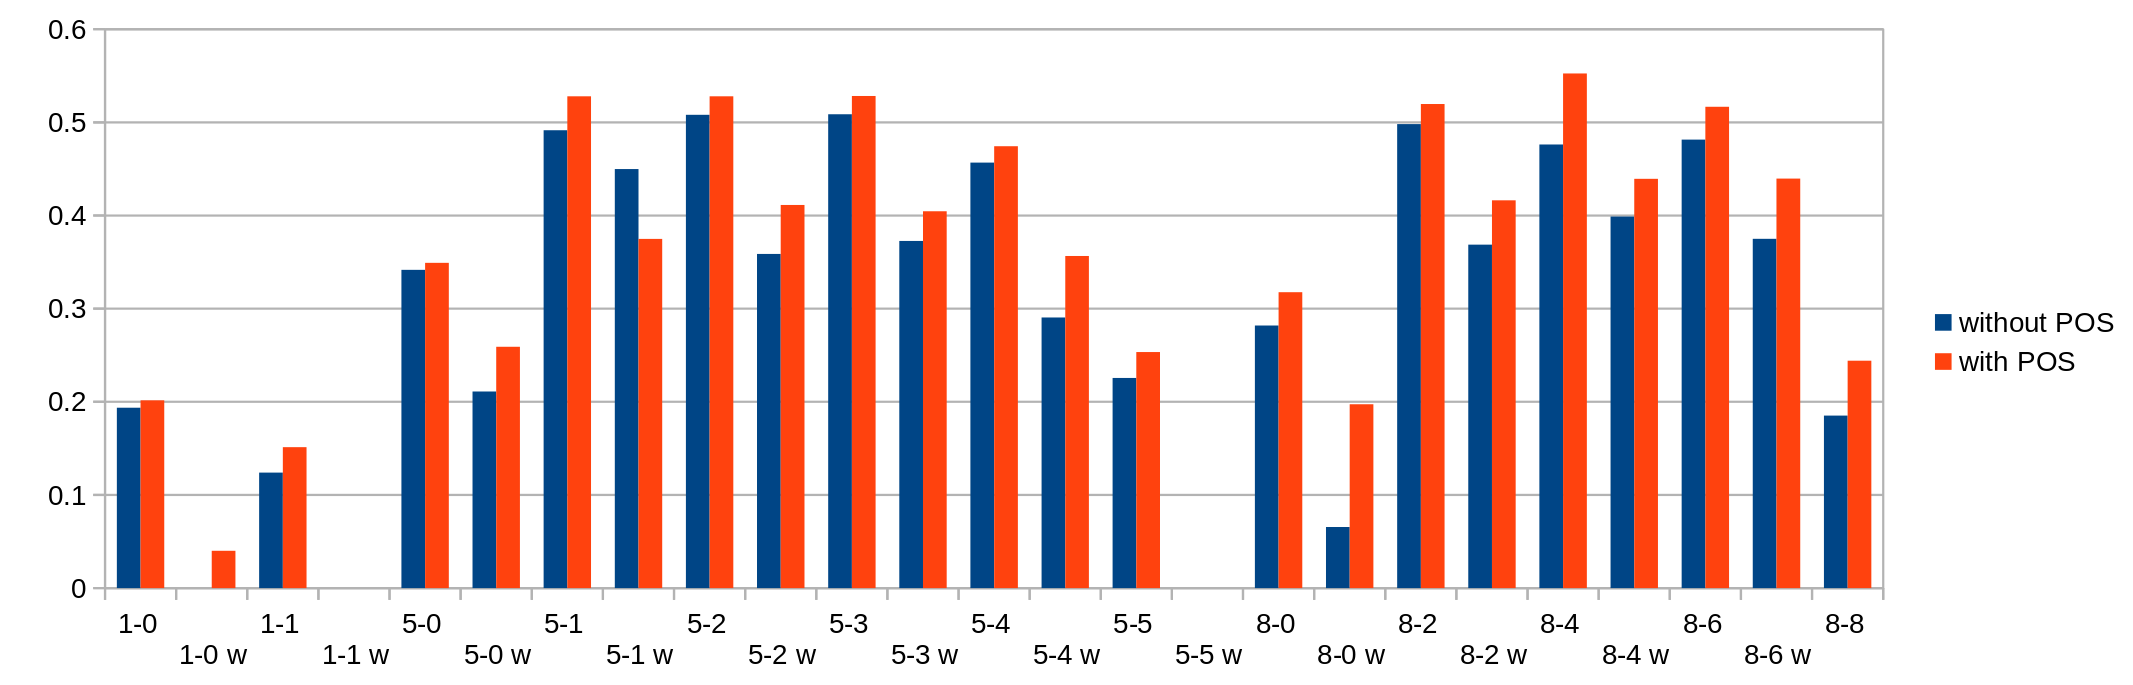
\includegraphics[width=\textwidth]{img/window_eval.png}
    \caption{Harmonic mean between all f1 scores for all classes. \emph{2/5} means window size of five and punctuation is tested at position two. If \emph{wi} is in the label, it uses wikipedia training data.}
    \label{window_eval}
\end{figure}

\begin{figure}[ht]
    \centering
    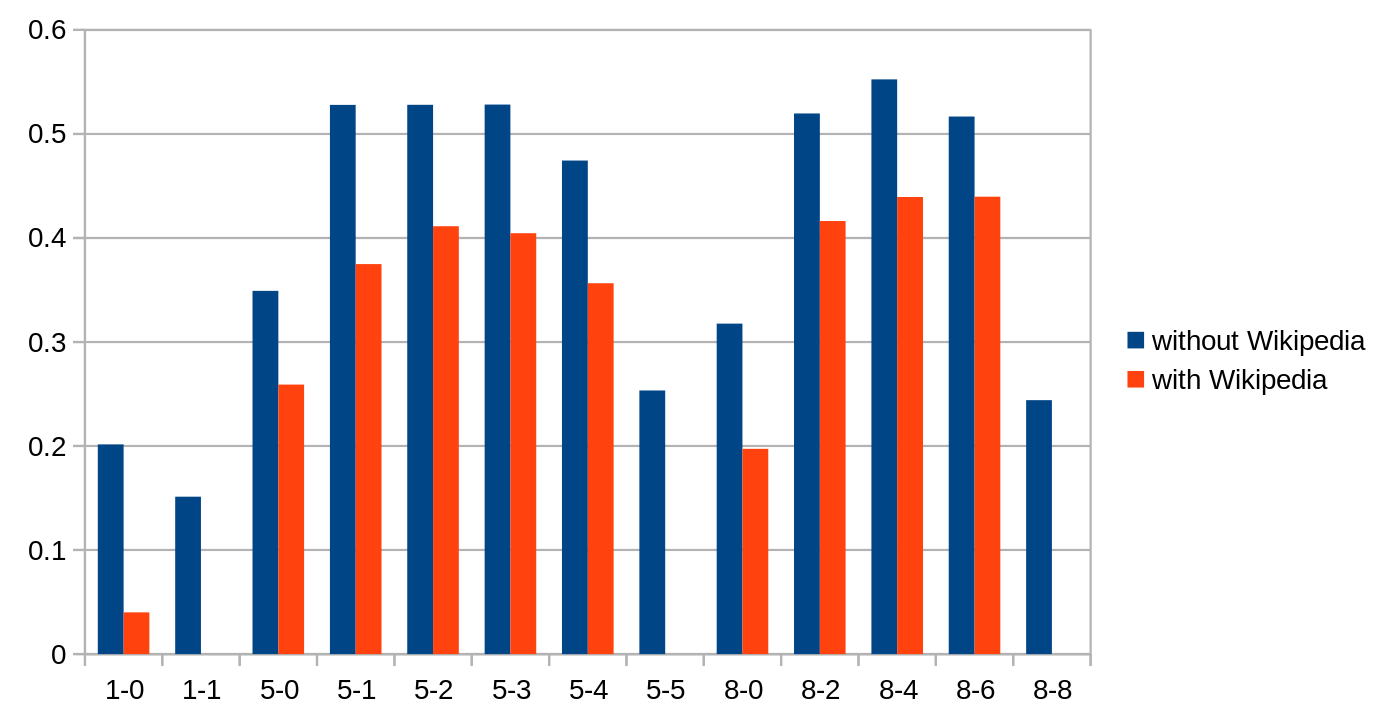
\includegraphics[width=\textwidth]{img/window_wiki_eval.png}
    \caption{}
    \label{window_wiki_eval}
\end{figure}

\begin{figure}[ht]
    \centering
    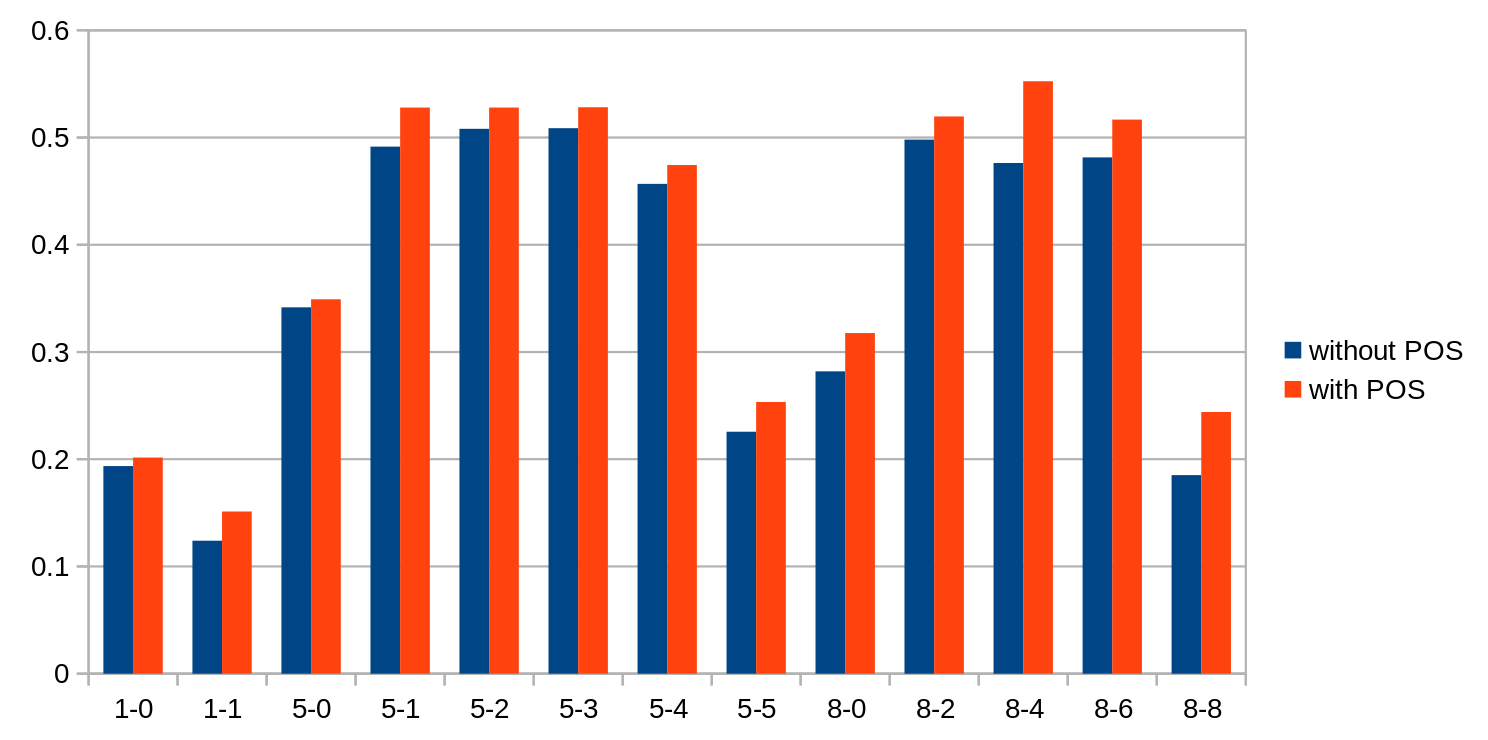
\includegraphics[width=\textwidth]{img/window_pos_eval.png}
    \caption{}
    \label{window_pos_eval}
\end{figure}

Comparison between experiments with and without POS tagging (other than that, they have the same configurations):
\begin{itemize}
\item With POS tagging: 0.305
\item Without POS tagging: 0.275
\end{itemize}

Comparison between experiments with and without wikipedia data (other than that, they have the same configurations):
\begin{itemize}
\item Without wikipedia: 0.385
\item With wikipedia data: 0.252
\end{itemize}
